\documentclass[letterpaper]{article}

% --- Packages
\usepackage[utf8]{inputenc}
\usepackage[T1]{fontenc}
\usepackage[margin=0.25cm]{geometry}
\usepackage{enumitem}
\usepackage{pdfpages}
\usepackage{multicol}
\usepackage{amsmath}
\usepackage{amssymb}
\usepackage[skip=1pt plus1pt, indent=0pt]{parskip}
\usepackage{enumitem}
\usepackage{graphicx}

% --- Data
\title{Complex Analysis}
\author{Enrique Calderon}
\date{October 2023}

% --- Graphics path
\graphicspath{ {./img/} }

% --- Custom commands
\makeatletter
\let\thetitle\@title
\let\theauthor\@author
\makeatother
\newcommand{\compconj}[1]{%
	\overline{#1}%
}
\newcommand{\divline}{\noindent\makebox[\linewidth]{\rule{\textwidth}{0.4pt}}}
\newcommand{\taninv}{\tan^{-1}}

\begin{document}
        \maketitle

        \divline

	\begin{multicols}{3}
		\section{Basic operators}
		
			Complex Number:
			\[z = x + iy\]
			
			Addition and subtraction:
			\[z_1 \pm z_2 = (x_1 \pm x_2) + i(y_1 \pm y_2)\]
			
			Product:
			\[z_1 \cdot z_2 = [(x_1 \cdot x_2) - (y_1 \cdot y_2)] + i[(x_1 \cdot y_2) + (y_1 \cdot x_2)]\]
			
			Conjugate:
			\[z \cdot \compconj{z} = (x + iy)(x - iy) = x^{2} + y^{2}\]
			
			Division:
			\[\frac{z_1}{z_2} = \frac{x_1 x_2 + y_1 y_2}{x_2^{2} + y_2^{2}} + i \frac{x_1 y_2 + x_2 y_1}{x_2^{2} + y_2^{2}}\]
			
			Power:
			\[z^{w} = e^{w \cdot \log{z}} \quad | \quad \forall \quad z,w \in \mathbb{C}\]

			Logarithm:
			\[\log{z} = \ln{|z|} + i \cdot \taninv{\frac{y}{x}}\]
			\[\ln{|z|} = \ln(r) + i\ln(\theta + 2kr)\]
			
			Exponential product:
			\[z_1 \cdot z_2 = r_1 e^{i\theta_1} \cdot r_2 e^{i\theta_2} \]
			
			Exponential division:
			\[\frac{z_1}{z_2} = \frac{r_1 e^{i\theta_1}}{r_2 e^{i\theta_2}} = \frac{r_1}{r_2} \cdot e^{i(\theta_1 - \theta_2)}\]
			
			Exponential root:
			\[\sqrt[n]{z} = (z)^{\frac{1}{n}} = r^{\frac{1}{n}} \cdot e^{i[\frac{\theta + 2kr}{n}]}\]
			
			Where there are n roots, \(k = 0, 1 , 2 , ... , n-1\)
	\end{multicols}
 
	\divline
 
	\begin{multicols}{3}
		\section{Set}
			The module if z is \(|z|\), where \(z \in \mathbb{R}\)
			
			Circumference with radius \(k\):
			\[|z + z_0| = k\]
			
			To the set \(z\) that exists near the point we know it as \textbf{Neighborhood} with radius \(\rho\)
			\[z - z_0 = \rho\]
			
			\textit{\textbf{Points}}
			
			\begin{itemize}
				\item \textit{Frontier}: Point which neighborhood is both inside and outside \(z\)
				\item \textit{Interior}: Point which neighborhood is only inside \(z\)
			\end{itemize}
			
			\textit{\textbf{Sets}}
			
			\begin{itemize}
				\item \textit{Open}: Exclusively of interior points
				\item \textit{Closed}: Inner and frontier points, is limited by \(\mathbb{R}\) and \(\mathbb{C}\)
				\item \textit{Neither open nor closed}
			\end{itemize}
	\end{multicols}
 
	\divline
 
	\begin{multicols}{3}
		\section{Complex functions}
			\textbf{Linear mapping}
				\[f(z) = az + b\]
				
				For a, \(r\) modifies magnitude and \(\theta\) the angle:
				\[f(z) = az = (r_ae^{i\theta_a}) \cdot (re^{i\theta}) = (r_ar) \cdot (e^{i(\theta_a + \theta)})\]
				
				For b, \(\mathbb{R}(b)\) move in \(\mathbb{R}\) and \(\mathbb{I}(b)\) move in \(\mathbb{I}\):
				\[f(z) = z + b\]

			\textbf{Potential mapping}
				\[f(z) = z^{n}\]
				
				\(f(z) = z^{2}\) : \(x = k\) and \(y = k\) generate parabolas.
				
				\(f(z) = z^{3}\) : generate curves.
			
			\textbf{Inverse mapping}
			
				\[f(z) = \frac{1}{z} = \frac{1}{r} \cdot e^{-i\theta}\]
	\end{multicols}
 
	\divline
 
	\begin{multicols}{3}
		\section{Trigonometry}
			\[\cos{(z)} = \frac{e^{iz} + e^{-iz}}{2}\]
			\[\cos{(iz)} = \cosh{(z)}\]
			\[\cosh{(z)} = \frac{e^{-z} + e^{z}}{2}\]
			\[\sin{(z)} = \frac{e^{iz} - e^{-iz}}{2}\]
			\[-\sin{(iz)} = \sinh{(z)}\]
			\[\sinh{(z)} = \frac{e^{z} - e^{-z}}{2}\]
			\[e^{z} = e^{x + iy} = e^{x} \cdot (\cos(y) + isin(y))\]
			\[e^{iz} = e^{ix - y} = e^{-y} \cdot (\cos(x) + isin(x))\]
	\end{multicols}
 
	\divline
 
	\begin{multicols}{2}
		\section{Limits}
			Infinite possible directions, if not all the directions converge in the same point, the limit does not exist.
			
			\[\lim_{z \to z_0} = f(z) = f(z_0)\]
	\end{multicols}
 
	\divline
 
	\begin{multicols}{2}
		\section{Derivative}
			\[f'(z) = \lim_{\Delta z \to 0} \frac{u(x + \Delta x, y + \Delta y) + iv(x + \Delta x, y + \Delta y) - [u(x,y) + iv(x,y)]}{\Delta x + i \Delta y} \]
			
			Horizontally, \(\Delta z = \Delta x\) and \(\Delta y = 0\):
			\[f'(z) = \frac{\delta u(x,y)}{\delta x} + i\frac{\delta v(x,y)}{\delta x}\]
			
			Vertically, \(\Delta z = \Delta y\) and \(\Delta x = 0\):
			\[f'(z) = -i \frac{\delta u(x,y)}{\delta y} + \frac{\delta v(x,y)}{\delta y}\]
			
			Exponential:
			\[f'(z) = \frac{1}{r} e^{-i\theta} \left[\frac{\delta v}{\delta \theta} -i \frac{\delta u}{\delta \theta}\right]\]
			
			Multiple:
			\[f''(z) = \frac{\delta^{2} u}{\delta x^{2}} + \frac{\delta^{2} v}{\delta x^{2}} \text{ or } \frac{\delta^{2} u}{\delta y^{2}} + \frac{\delta^{2} v}{\delta y^{2}} \text{ or } \frac{\delta^{2} u}{\delta x \delta y} + \frac{\delta^{2} v}{\delta x \delta y} \] 
	\end{multicols}
 
	\divline
 
	\begin{multicols}{3}
		\section{Cauchy - Riemann}
		\[\frac{\delta u}{\delta x} = \frac{\delta v}{\delta y} \text{ and } \frac{\delta v}{\delta x} = - \frac{\delta u}{\delta y}\]
		
		If and only if \(f(z)\) is continuous in the domain \(D\) and C-R is true, them \(f(z)\) is analytic in D.
		
		If it is analytic, then  it is derivable in the same region. Once a function is harmonic, it is conjugate if C-R is true.
	\end{multicols}
 
	\divline
 
	\begin{multicols}{2}
		\section{Laplace}
			If \(f(z)\) is analytic in a region R and Laplace is true in the same region, the function is harmonic.
		
			Binomial:
			\[\frac{\delta^{2} u}{\delta x^{2}} + \frac{\delta^{2} u}{\delta y^{2}} = 0 \text{ and } \frac{\delta^{2} v}{\delta x^{2}} + \frac{\delta^{2} v}{\delta y^{2}} = 0\]
			
			Exponential:
			\[\frac{\delta^{2} u}{\delta r^{2}} + \frac{1}{r^{2}} \frac{\delta^{2} u}{\delta \theta^{2}} + \frac{1}{r} \frac{\delta u}{\delta \theta}\]
			
			\[\frac{\delta^{2} v}{\delta r^{2}} + \frac{1}{r^{2}} \frac{\delta^{2} v}{\delta \theta^{2}} + \frac{1}{r} \frac{\delta v}{\delta \theta}\]
	\end{multicols}
 
	\divline
 
	\begin{multicols}{2}
		\section{Integral}
			In analytic functions the calculus fundamental theorem is true but in non analytic there is a infinity of results.
			
			\[\int_{c}f(z)dz = \int_{t1}^{t2}f(z(t)) \cdot z'(t) dt\]
			
			If \(C\) contains \(z_0\):
			
			\[\oint_{c}\frac{1}{(z-z_0)^n}dz = 
				\begin{cases} 
					2 \pi i & n = 1 \\
					0 & n \geq 2
				\end{cases}
			\]
			
			\textbf{Cauchy theorem}
			
			\[\oint_{c} f(z)dz = \oint_{c_1}f(z)dz + \oint_{c_2}f(z)dz + ... + \oint_{c_n-1}f(z)dz\]
			
			If there are no discontinuities in C, the integral is 0. If there are discontinuities:
			
			\[\oint_{c}^{1}\frac{1}{z-z_0}dz = 2 \pi i\]
			
			If \(f(z)\) is analytic except in \(z = z_0\)
			
			\[f(z) = \frac{g(z)}{z - z_0} \to \oint_{c1}f(z)dz = 2 \pi i \cdot g(z) |_{z=z_0}\]
			
			For indeterminate, we get the singularity order, \(n\), which is the times we need to derive in order to get rid off the indeterminate. 
			
			\[\oint f(z)dz = \oint \frac{g(z)}{(z-z_0)^{n}} = \frac{2 \pi i}{(n-1)!} \cdot \frac{\delta^{n-1}}{\delta z^{n-1}} g(z) |_{z=z_0} \]			
	\end{multicols}
 
	\divline
 
	\begin{multicols}{2}
		\section{Series and successions}
			\textbf{Succession}
			
			Function with integers as domain.
			
			\textit{Convergence} : \(\lim_{n \to \infty} z_n = a + ib\)
			
			\textit{Cauchy criteria} : \(|z_n-z_m| < \epsilon\)
			
			\textbf{Series}
			
			Sum of a succession 
			
			\[\sum_{n=1}^{\infty} {z_n}\]
			
			\textit{Geometric function} : 
			
			\[\sum_{n=1}^{\infty} az^{n-1} = a + az + az^{2} + ...\]
			
			\textit{Series convergence} : 
			
			\[S_k = \frac{a(1-z^{k})}{(1-z)}\]
			
			\[\lim_{k \to \infty} z^k 
				\begin{cases}
					|z| > 1 \to z^{k} \to \infty \text{ so it diverges} \\
					|z| < 1 \to z^{k} \to 0 \text{ so it converges}
				\end{cases}
			\]
			
			So if \(|z| < 1\), it is convergent in \(S_k = \frac{a}{1-z}\)
			
			\textbf{Series}:
			
			\[ \frac{1}{1+z} = 1 - z + z^{2} - z^{3} + ... \]
			\[ \frac{1}{1-z} = 1 + z + z^{2} + z^{3} + ... \]
			\[ e^{z} = 1 + z + \frac{1}{2!} z^{2} + \frac{1}{3!} z^{3} + ... \]
			\[sen(z) = z - \frac{z^{3}}{3!} + \frac{z^{5}}{5!} + ... \]
			\[cos(z) = 1 - \frac{z^{2}}{2!} + \frac{z^{4}}{4!} + ... \]
			
			\textbf{Convergence criteria}:
			
			The proportion criteria
			\[
				\lim_{n \to \infty} \frac{| Z_{n+1} |}{| Z_n |}
			\]
			
			The root criteria
			\[
			\lim_{n \to \infty} \sqrt[n]{|Z_{n}|}
			\]
			
			Where:
			
			\[
			\begin{cases}
				L < 1 \to \text{ converges} \\
				L > 1 \to \text{ diverges} \\
				L = 1 \to \text{ unknown} \\
			\end{cases}
			\]
			
			Power series:
			
			\[ \sum_{n = 0}^{\infty} a_{n} (z - z_0)^{n} = a_0 + a_{1}(z-z_0) +a_{2}(z-z_0)^{2} + ... \]
			
			We can use root or proportion criteria with \(a_{n}\) to determine the convergence
			
			Convergence radio, in power series \(a_{n}\) is the coefficient and \(z_0\) the center of the series. It is important because there the equality is true, to calculate it:
			
			\[R = \frac{1}{L}\]
			
			\[a_n = \frac{1}{n!} \cdot \frac{\delta^{n}}{\delta z^{n}} f(z) |_{z=z_0} \]
			
			\textbf{Taylor}: in a point.
			
			\textbf{Maclaurin}: in origin.
			
			\textbf{Laurent}:
			
			\[f(z) = ... + \frac{a_{-k}}{(z-z_0)^{k}} + ... + \frac{a_{-1}}{z-z_0} + a_0 + a_{1}(z-z_0) + ...\]
			
			Where the principal part is:
			
			\[... + \frac{a_{-k}}{(z-z_0)^{k}} + ... + \frac{a_{-1}}{z-z_0}\]
			
			And the analytic part is:
			
			\[a_0 + a_{1}(z-z_0) + ...\]
			
			To obtain \(a_k\):
			
			\[a_k = \frac{1}{2 \pi i} \oint_{c} \frac{f(z)}{(z-z_0)^{k+1}} dz \]
			
	\end{multicols}
 
	\divline
 
	\begin{multicols}{2}
		\section{Residue theory}
				By theory:
		
			\[Res(f, z_0) = \lim_{z \to z_0} \frac{1}{(k-1)!} \frac{\delta^{k-1}}{\delta z^{k-1}} [(z-z_0)^{k}f(z)])\]
			
			The residue of \(f(z)\) in \(z = z_0\) is:
			
			\[a_{-1} = \frac{1}{2 \pi i} \oint f(z)dz \]
			
			In a curve with \(N\) discontinuities:
			
			\[\oint_{c} f(z)dz = 2 \pi i \cdot \sum_{k = 1}^{N} \text{Res} \{f(z), z = z_0)\}\]
	\end{multicols}
            \begin{center}
                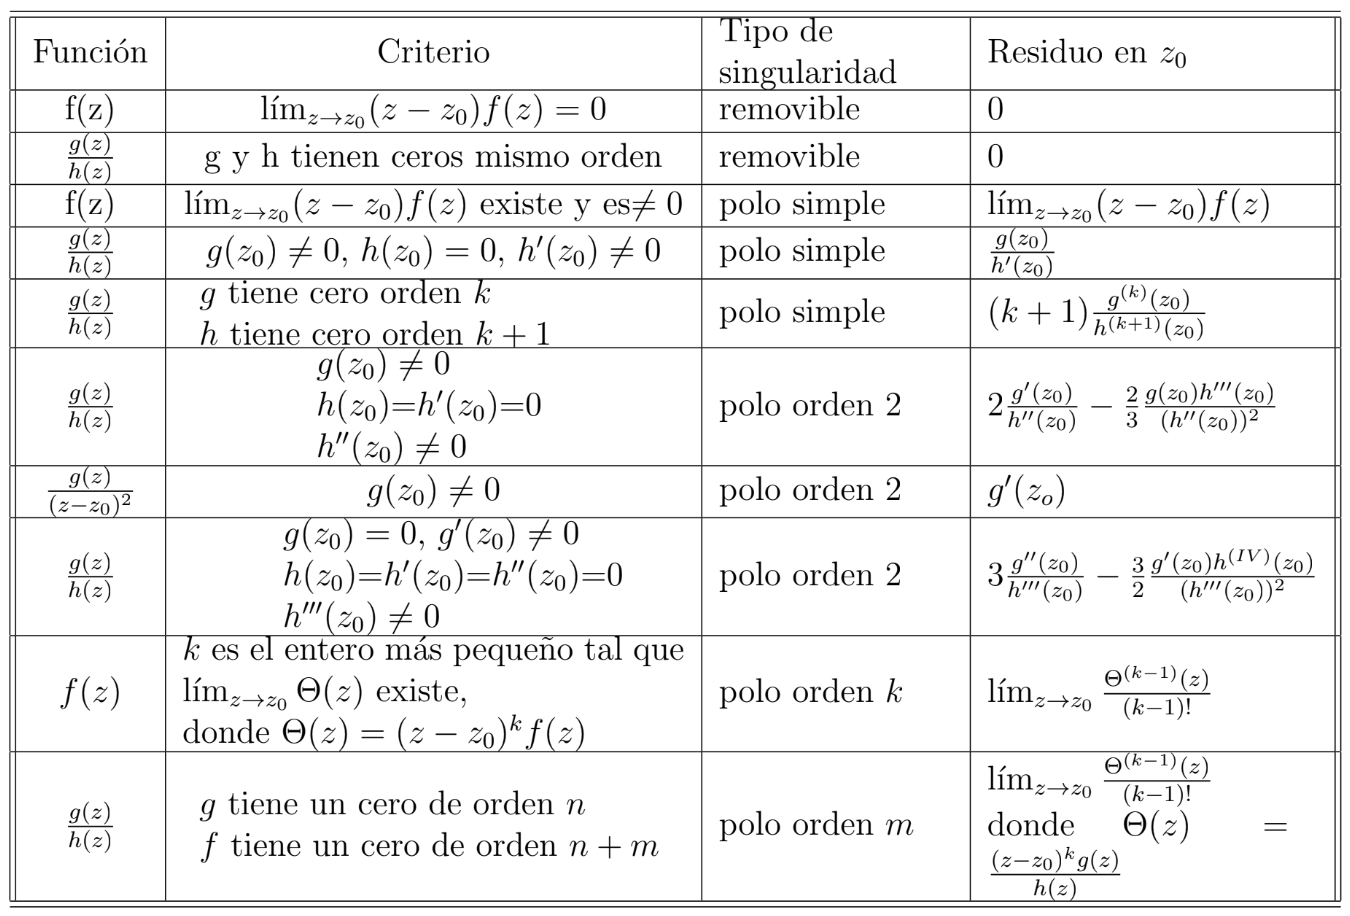
\includegraphics[width=0.8\textwidth]{ResidueTable}
            \end{center}
\end{document}
